\documentclass[a4paper]{article}
% Brug denne, hvis der kun printes på den ene side!
%\documentclass[a4paper]{article}
\usepackage[utf8]{inputenc}
\usepackage{amsmath}
\usepackage{amsfonts}
\usepackage{amssymb}
\usepackage{graphicx}
\usepackage{subfiles}
\usepackage{gensymb}
\usepackage{float}
\usepackage{wrapfig}
\usepackage{bm}
\usepackage[backend=biber,style=numeric,sorting=none]{biblatex} % Package for bibliography (citing)
\addbibresource{bibliography.bib}

% geometry-pakken bruges til f.eks. at ændre margnerne.
% Gør ikke margnerne smallere end dette - Jakob bliver ikke glad!
\usepackage[rmargin=3.2cm,tmargin=3.5cm]{geometry}
% Disse to linjer sikrer, at der bliver mellemrum i stedet for indrykning ved afsnit
\setlength{\parindent}{0pt}
\setlength{\parskip}{1ex plus 0.5ex minus 0.2ex}
\usepackage{caption}
\usepackage{subcaption}
\usepackage[table,xcdraw]{xcolor}
\usepackage{gensymb}
\usepackage{multirow}
\usepackage{pdfpages}

% Her begynder selve dokumentet
\begin{document}
% titlepage-miljøet bruges til at sætte en forside op og gør blandt andet at der ikke kommer sidetal
% på og at der automatisk bliver skiftet til en ny side når den er færdig
% At opsætte en forside manuelt kan godt blive lidt kompliceret at se på og man vil derfor ofte
% rykke kode som dette ud i en seperat fil f.eks. forside.tex og inkludere den her med \input{forside}
\begin{titlepage}
\centering
% For forklaring af vspace og stretch, se side 115 i ".. not so short .."
% www.ctan.org/tex-archive/info/lshort/english/lshort.pdf
\vspace*{\stretch{1}}
% rule laver en linje på tværs af siden
\rule{\textwidth}{1mm}\\
\vspace{1cm}
% Her vælger en kæmpe skrifttype og fed skrift
\Huge\bfseries DGFEM Formulation of spherical Linear Shallow Water Equations\\
\vspace{0.7cm}
\rule{\textwidth}{1mm}\\
\vspace{3cm}
\large
Simon Bjerre (s224059) \\
\vspace{1.7cm}

\vspace*{\stretch{2}}
% Nulstiller skriftstørrelse og type (f.eks. fed)
\normalsize
\begin{flushleft}
Report for special course.\\
Danmarks Tekniske Universitet\\

\end{flushleft}
\end{titlepage}
\tableofcontents

% \input{Afsnit/Notation}
\newpage
\section{Cartesian formulation (flat)}\label{sec:flat}
We define a region $\Omega$, $h$ is the height of the water column, and we assume hydrostatic pressure. The bottom is at the elevation $b(x,y)$ above the reference level $z = 0$, the mean sea level, and the free surface is at the elevation $\zeta = h + b$. We denote the velocity vector as $\mathbf{u}$, the outward normal on the domain as $\hat{\mathbf{n}}$, and the local vertical is $\hat{\mathbf{k}}$.

% ---------------------------------------------------------------------
\subsection{Mass conservation}\label{sec:car-Mass}
Using the density $\rho$ we can write the mass per unit area: $\rho h$. So the total mass in $\Omega$ is then:
\begin{equation*}
    \int_\Omega\rho h\,dA
\end{equation*}
We assume $\rho = 1$ and constant. Since the bottom does not move in time, only the height of the water column changes the mass in $\Omega$. We know that mass is conserved: the change of mass inside the domain should be equal to the net mass flowing out of the boundary of the domain. We write this as:
\begin{equation*}
    \frac{d}{dt}\int_\Omega\rho h\,dA = -\oint_{\partial\Omega}(h\mathbf{u})\cdot\hat{\mathbf{n}}\,dS
\end{equation*}
We use the divergence theorem:
\begin{equation*}
    \frac{d}{dt}\int_\Omega h\,dA = -\oint_{\partial\Omega}(h\mathbf{u})\cdot\hat{\mathbf{n}}\,dS = -\int_\Omega\nabla\cdot(h\mathbf{u})\,dA
\end{equation*}
Rearranging:
\begin{equation}\label{eq:flat-mass-integral}
    \int_\Omega\frac{\partial h}{\partial t} + \nabla\cdot(h\mathbf{u})\,dA = 0
\end{equation}
The integral vanishes for every $\Omega$. Suppose the integrand is non-zero at a point $p$, say positive. Choose $\Omega$ to be a small disc around $p$; then the integral is positive, so for eq.~\eqref{eq:flat-mass-integral} to hold we need:
\begin{equation}\label{eq:flat-mass}
    \frac{\partial h}{\partial t} + \nabla\cdot(h\mathbf{u}) = 0
\end{equation}
This is our mass conservation.

% ---------------------------------------------------------------------
\subsection{Momentum conservation}
Now for the momentum conservation, we have:
\begin{equation}\label{eq:flat-momentum}
    \frac{d}{dt}\int_\Omega h\mathbf{u}\,dA = -\oint_{\partial\Omega}(\text{momentum flux})\cdot\hat{\mathbf{n}}\,dS + \text{force}
\end{equation}

\paragraph{Momentum flux}
There are two parts of the flux:

Advective:
\begin{equation*}
    h\mathbf{u}\otimes\mathbf{u}
\end{equation*}
Pressure: We assume hydrostatic balance, so the pressure at the bottom is $\rho gh$. Integrating from the bottom to the surface:
\begin{equation*}
    \int_b^{b+h}\rho g(b + h - z)\,dz = \frac12\rho gh^2 \quad\Rightarrow\quad \frac12gh^2
\end{equation*}
The integrated pressure only depends on the height of the water column, not on the elevation of the bottom. Pressure in a fluid acts equally in all directions, so the pressure term is:
\begin{equation*}
    \frac12gh^2\mathbf{I}
\end{equation*}
The momentum flux tensor is:
\begin{equation}\label{eq:flat-flux}
    \mathbf{F} = h\mathbf{u}\otimes\mathbf{u} + \frac12gh^2\mathbf{I}
\end{equation}

Thus we have our SWEs in a flat domain in Cartesian formulation. For $\mathbf{u} = 0$ the momentum equation reduces to $\nabla(\frac12gh^2) + gh\nabla b = gh\nabla(h + b) = 0$, so a fluid at rest with a flat free surface, $h + b$ constant, is a steady state. This is the lake at rest, which is discussed on the sphere in section \ref{sec:sph-rest}.

\section{Ambient spherical formulation}
We define a region $\Omega$ on the sphere of radius $R$, $h$ is the height of the water column, and we assume hydrostatic pressure. The bottom is at the elevation $b(\mathbf{x})$ above the sphere, which is the mean sea level, so $b<0$ in the ocean and $b>0$ on land, and the free surface is at the elevation $\zeta = h + b$. We denote the velocity vector as $\mathbf{u}$, the outward normal on the domain as $\hat{\mathbf{n}}$ and the outward normal for the sphere as $\mathbf{n}$.

% ---------------------------------------------------------------------
\subsection{Mass conservation}
We use the same observations about mass as in the Cartesian formulation: mass is conserved, so the change of mass inside the domain should be equal to the net mass flowing out of the domain. Since the bottom does not move in time, the bathymetry does not enter the mass balance. We then go on to apply the divergence theorem, but now we are on a curved surface, where the divergence theorem is given by (see p.~297, Th.~2.10 in \cite{Dziuk_Elliott_2013}):
\begin{equation}\label{eq:sph-divthm}
    \int_\Omega\nabla_s\cdot(h\mathbf{u})\,dA = \oint_{\partial\Omega}(h\mathbf{u})\cdot\hat{\mathbf{n}}\,dS + \int_\Omega H\,(h\mathbf{u})\cdot\mathbf{n}\,dA
\end{equation}
where $H = \nabla_s\cdot\mathbf{n} = 2/R$ is the total curvature for a sphere. Because $h\mathbf{u}$ is tangential, the last term on the right hand side of eq.~\eqref{eq:sph-divthm} is zero, therefore we have the same mass conservation as in Cartesian coordinates:
\begin{equation*}
    \frac{\partial h}{\partial t} + \nabla_s\cdot(h\mathbf{u}) = 0
\end{equation*}
This is our mass conservation.

% ---------------------------------------------------------------------
\subsection{Momentum conservation}
Now for the momentum conservation, it is the same considerations as for the Cartesian coordinates (eq.~\ref{eq:flat-momentum}).

\paragraph{Momentum flux}
There are still advective and pressure terms in spherical coordinates. The bottom does not change the pressure in the column: it is still hydrostatic, $p = g(R + b + h - r)$ for $R + b\leq r\leq R + b + h$, where $r = |\mathbf{x}|$ is the distance from the centre of the Earth, so integrating from the bottom to the surface gives $\frac12gh^2$, as in section 2. The advective term is already fine on the curved surface. But in order for the pressure term to be correctly defined on the curved surface we need the divergence theorem to hold, and it only holds if each row of the tensor it is applied to is tangential. This means that $\mathbf{T}\mathbf{n} = 0$ for a tensor $\mathbf{T}$. For the two terms of the flux tensor defined in Cartesian coordinates (eq.~\ref{eq:flat-flux}) we have:
\begin{itemize}
    \item Advective: $(h\mathbf{u}\otimes\mathbf{u})\mathbf{n} = h\mathbf{u}(\mathbf{u}\cdot\mathbf{n}) = 0$
    \item Pressure: $\mathbf{I}\mathbf{n} = \mathbf{n}\neq0$
\end{itemize}
We need the tensor to be tangential, therefore we use the projection operator $\mathbf{P} = \mathbf{I} - \mathbf{n}\mathbf{n}^T$ instead of the identity operator. This can be done because the operators agree on the boundary, since $\mathbf{I}\hat{\mathbf{n}} = \hat{\mathbf{n}} = \mathbf{P}\hat{\mathbf{n}}$. We want the boundary integrand to be unchanged, therefore the pressure term of the flux is
\begin{equation*}
    \frac12gh^2\mathbf{P}.
\end{equation*}
We write the momentum flux tensor:
\begin{equation}\label{eq:sph-flux}
    \mathbf{F} = h\mathbf{u}\otimes\mathbf{u} + \frac12gh^2\mathbf{P}
\end{equation}

% ---------------------------------------------------------------------
\subsection{The SWEs in ambient spherical formulation}
Using the results from the above sections we get our SWEs in spherical formulation:
\begin{align}
    \frac{\partial h}{\partial t} + \nabla_s\cdot(h\mathbf{u}) &= 0 \label{eq:system1}\\
    \frac{\partial}{\partial t}(h\mathbf{u}) + \nabla_s\cdot\mathbf{F} &= -2\boldsymbol{\omega}\times(h\mathbf{u}) - gh\nabla_s b + \lambda\mathbf{n} \label{eq:system2}
\end{align}
where $\mathbf{F} = h\mathbf{u}\otimes\mathbf{u} + \frac12gh^2\mathbf{P}$ and $\lambda = -\frac{h|\mathbf{u}|^2}{R} - \frac{gh^2}{R} + 2h\,\mathbf{n}\cdot(\boldsymbol{\omega}\times\mathbf{u})$. For a flat bottom the bathymetry term vanishes.

% ---------------------------------------------------------------------
\subsection{Lake at rest and wave speed}\label{sec:sph-rest}
Here we take a lot of inspiration from \cite{bonev2018discontinuous}, they use the lake at rest as a steady-state solution for which the scheme needs to be well-balanced, we use the same test for our scheme and equations in order to see if we are on the right track.

\paragraph{Lake at rest}
A fluid at rest with a flat free surface, $\mathbf{u} = 0$ and $h + b = \zeta_0$ constant, is a steady state of eqs.~\eqref{eq:system1}--\eqref{eq:system2}. The mass equation is satisfied since $h\mathbf{u} = 0$. In the momentum equation the advective and Coriolis terms vanish, and with the pressure term eq.~\eqref{eq:sph-pressure} and $\lambda = -gh^2/R$ for $\mathbf{u} = 0$, it reads
\begin{equation*}
    gh\nabla_s h - \frac{gh^2}{R}\mathbf{n} = -gh\nabla_s b - \frac{gh^2}{R}\mathbf{n}
    \quad\Leftrightarrow\quad gh\nabla_s(h + b) = 0,
\end{equation*}
which holds since $h + b = \zeta_0$. The normal parts balance each other, and in the tangential part the pressure gradient balances the bottom force. This steady state is called the lake at rest \cite{bonev2018discontinuous}. A tsunami is a small perturbation of it, while the two balanced terms can be large. Over a continental slope with the gradient $0.05$ in $4000$ m of water, $gh|\nabla_s b|\approx2000$ m$^2$/s$^2$, whereas a tsunami with the amplitude $1$ m and the wavelength $500$ km has $gh|\nabla_s\zeta|\approx0.5$ m$^2$/s$^2$. A relative error of a few times $10^{-4}$ in the balance is thus as large as the tsunami itself. A numerical scheme must therefore preserve the lake at rest exactly, i.e.\ be well-balanced, otherwise the discretization errors of the two balanced terms produce spurious waves. We return to this in section 4.

% ========================================================================
\subsection{Advection on the sphere}\label{sec:sph-advection}
Before solving the SWEs we test the scheme on the simplest equation of the same form: the transport of the height $h$ by a prescribed tangential velocity field $\mathbf{v}(\mathbf{x})$. This is the mass equation \eqref{eq:system1} with $\mathbf{u}$ replaced by $\mathbf{v}$, and the momentum equation removed,
\begin{equation}\label{eq:advection}
    \frac{\partial h}{\partial t} + \nabla_s\cdot(h\mathbf{v}) = 0 .
\end{equation}
In the form of eq.~\eqref{eq:conservation} this is $q = h$, $\mathbf{F}(q) = h\mathbf{v}$ and $S = 0$. Since $\mathbf{v}$ does not depend on $h$, the equation is linear, and its only wave speed is the transport speed $|\mathbf{v}|$.

Following test case 1 of \cite{williamson1992standard} we use a solid-body rotation about an axis $\mathbf{e}$, tilted by the angle $\alpha$ from the polar axis,
\begin{equation}\label{eq:sbr}
    \mathbf{v} = \frac{u_0}{R}\,\mathbf{e}\times\mathbf{x}, \qquad
    \mathbf{e} = (-\sin\alpha,\, 0,\, \cos\alpha), \qquad
    u_0 = \frac{2\pi R}{12\ \text{days}} .
\end{equation}
The field is tangential, $\mathbf{v}\cdot\mathbf{n} = (\mathbf{e}\times\mathbf{x})\cdot\mathbf{x}/R^2 = 0$, and divergence free, $\nabla_s\cdot\mathbf{v} = 0$, so eq.~\eqref{eq:advection} reduces to $\partial_t h + \mathbf{v}\cdot\nabla_s h = 0$: the initial field is rotated rigidly about $\mathbf{e}$ and returns to its starting point after $12$ days. This gives an exact solution at all times. Varying $\alpha$ moves the path of the flow relative to the grid: $\alpha = 0$ is along the equator, while $\alpha = \pi/2$ passes directly over the poles.

The initial condition is the cosine bell
\begin{equation}\label{eq:cosinebell}
    h(\mathbf{x},0) =
    \begin{cases}
        \frac{h_0}{2}\left(1 + \cos\frac{\pi r}{R_b}\right), & r < R_b,\\
        0, & r \geq R_b,
    \end{cases}
    \qquad r = R\arccos\left(\frac{\mathbf{x}_c\cdot\mathbf{x}}{R^2}\right),
\end{equation}
with $h_0 = 1000$ m, $R_b = R/3$ and the centre $\mathbf{x}_c$ on the equator. The bell is only $C^1$: its second derivative jumps at $r = R_b$. We therefore expect algebraic rather than spectral convergence under $p$-refinement.
% ========================================================================

\subsection{Linearized SWEs}
We assume a flat bottom in this project and want to test on the linearized SWEs, therefore we first write the nonlinear equation:
$$
\frac{\partial q}{\partial t} + \nabla_s \cdot \mathbf{F}(q) = S(x,q)
$$
Since we assume a flat bottom, that the Coriolis has little influence on the test timescale of 40-60h and that the normal part is resolved by projecting onto the tangent plane we let $S(x,q)=0$. We linearize around the lake at rest with a flat bottom, $q_0$: $h_0 = D$, $\mathbf{u}_0 = 0$,
and neglect the Coriolis force. For the nonlinear case, Coriolis is kept in the model. We add a small perturbation,
\begin{equation*}
    h = D + \epsilon\zeta', \qquad \mathbf{u} = \epsilon\mathbf{u}', \qquad \epsilon \ll 1,
\end{equation*}
insert it in eqs.~\eqref{eq:system1}--\eqref{eq:system2} and collect powers of $\epsilon$.
The mass equation becomes
\begin{equation}\label{eq:LinearMass}
    \partial_t(D + \epsilon\zeta') + \nabla_s\cdot\big((D + \epsilon\zeta')\,\epsilon\mathbf{u}'\big)
    = \epsilon\big(\partial_t\zeta' + \nabla_s\cdot(D\mathbf{u}')\big) + \epsilon^2\,\nabla_s\cdot(\zeta'\mathbf{u}') = 0 .
\end{equation}
In the momentum equation the time derivative and the flux become
\begin{align}
    \partial_t(h\mathbf{u}) &= \epsilon\,\partial_t(D\mathbf{u}') + \epsilon^2\,\partial_t(\zeta'\mathbf{u}'), \label{eq:LinearMomentumTime}\\
    h\mathbf{u}\otimes\mathbf{u} + \tfrac12 gh^2\mathbf{I}
    &= \tfrac12 gD^2\mathbf{I} + \epsilon\, gD\zeta'\mathbf{I}
    + \epsilon^2\big(\tfrac12 g\zeta'^2\mathbf{I} + D\,\mathbf{u}'\otimes\mathbf{u}'\big) + \mathcal{O}(\epsilon^3). \label{eq:LinearMomentumFlux}
\end{align}
The $\epsilon^0$ terms vanish, since $\partial_t D = 0$ and $\nabla_s\cdot(\tfrac12 gD^2\mathbf{I}) = 0$ for constant $D$. We keep the $\mathcal{O}(\epsilon)$ terms, divide by $\epsilon$ and neglect $\mathcal{O}(\epsilon^2)$.
With $\mathbf{m} = D\mathbf{u}'$ we get the linear SWE
\begin{align}
    \partial_t\zeta + \nabla_s\cdot\mathbf{m} &= 0 \label{eq:LinearSys1},\\
    \partial_t\mathbf{m} + \nabla_s\cdot(gD\zeta\,\mathbf{I}) &= 0 \label{eq:LinearSys2}
\end{align}

\subsection{Exact Legendre Solution}
We test our linear solver with against an exact solution for the Gaussian bump on a sphere, the derivation for the exact solution can be found in the note at \cite{Note_Jayshree}. We modify the system in \eqref{eq:LinearSys1}, \eqref{eq:LinearSys2} by differentiating \eqref{eq:LinearSys1} in time and inserting \eqref{eq:LinearSys2}:
\begin{align*}
    \partial_{tt}\zeta + \nabla_s\cdot\partial_t\mathbf{m} = \partial_{tt}\zeta + \nabla_s\cdot(-\nabla_s\cdot(gD\zeta\mathbf{I})) \Rightarrow \\
    \partial_{tt}\zeta = gD\nabla_s\cdot(\nabla_s\cdot(\zeta\mathbf{I})) = gD\nabla_s\cdot(\nabla_s\zeta) = gD\Delta_s\zeta
\end{align*}
We see this is exactly the wave equation with $c^2=gD$.

In the full derivation spherical harmonics are used, however the Gaussian only depends on the angle $\alpha$ from its centre C. We let C be the pole, then only $m=0$ terms are kept. By rotating so the Gaussian bump sits on the pole, we can use Legendre polynomials for the exact solution. For the bump we use a width $\sigma = 800km$ and we truncate the Legendre series at $L=200$. 

In order to check if we get proper behaviour at the poles as expected with the mesh descriped below then we move our Gaussian off-center and let $\theta_0=30\degree N$ and $\phi_0 = 140\degree E$ in order to check if the wave moves over the north or south poles correctly


\section{Mesh}\label{sec:mesh}
To solve the SWEs on the sphere we need to cover the sphere with elements. A lat-lon grid seems like a good choice, but its grid lines converge at the poles, where the elements become very small and the explicit time step with them, and the poles are singular points. Instead we follow \cite{bonev2018discontinuous, GIRALDO2002499} and build a mesh of quadrilaterals from an icosahedron. It has no singular points, and all elements are roughly the same size.

\subsection{Construction}\label{sec:mesh-construction}
The mesh is built in four steps, controlled by one refinement parameter $n_I$.

\paragraph{Icosahedron}
The icosahedron has the 12 vertices $(0,\pm1,\pm\varphi)$, $(\pm1,\pm\varphi,0)$ and $(\pm\varphi,0,\pm1)$, where $\varphi = (1+\sqrt5)/2$, which we normalise to lie on the unit sphere. Its 20 faces are equilateral triangles, which we take from the convex hull of the vertices and order counter-clockwise seen from outside the sphere.

\paragraph{Subdivision}
Each face with the vertices $\mathbf{A}$, $\mathbf{B}$, $\mathbf{C}$ is divided into $n_I^2$ triangles through the points
\begin{equation*}
    \mathbf{p}_{ab} = \mathbf{A} + \frac{a}{n_I}(\mathbf{B}-\mathbf{A}) + \frac{b}{n_I}(\mathbf{C}-\mathbf{A}), \qquad a,b\in\{0,1,\dots,n_I\},\quad a+b\leq n_I
\end{equation*}

\begin{figure}[H]
    \centering
    \begin{subfigure}{0.32\textwidth}
        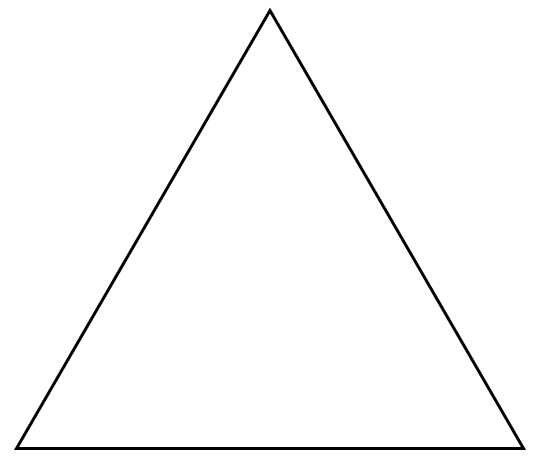
\includegraphics[width=\textwidth]{Figures/Sketches/Rough.png}
        \caption{Regular triangular face of the icosahedron}
    \end{subfigure}
    \hfill
    \begin{subfigure}{0.32\textwidth}
        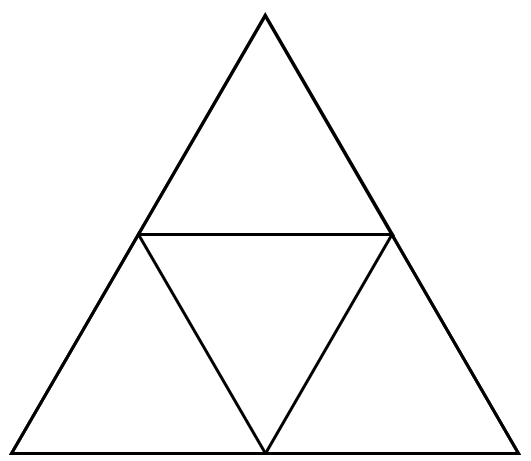
\includegraphics[width=\textwidth]{Figures/Sketches/Finer.png}
        \caption{Triangle refined to $n_I^2 = 2^2 = 4$ triangles}
    \end{subfigure}
    \hfill
    \begin{subfigure}{0.32\textwidth}
        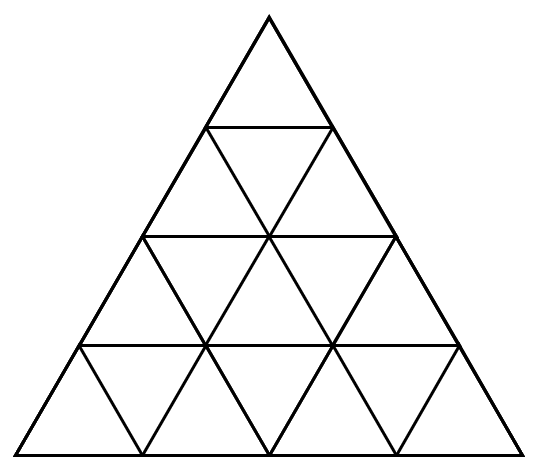
\includegraphics[width=\textwidth]{Figures/Sketches/Finest.png}
        \caption{Triangle refined to $n_I^2 = 4^2 = 16$ triangles}
    \end{subfigure}
    \caption{Refinement of the icosahedron faces}
    \label{fig:Tri_refine}
\end{figure}

\paragraph{Triangles to quadrilaterals}
Each small triangle is split into three quadrilaterals by connecting its centroid to the midpoints of its sides. Every quadrilateral has one vertex of the triangle, two midpoints and the centroid as vertices, ordered counter-clockwise. This gives
$K = 20\cdot n_I^2\cdot 3 = 60\,n_I^2 $ elements.
\begin{figure}[H]
    \centering
    \begin{subfigure}{0.48\textwidth}
        \centering
        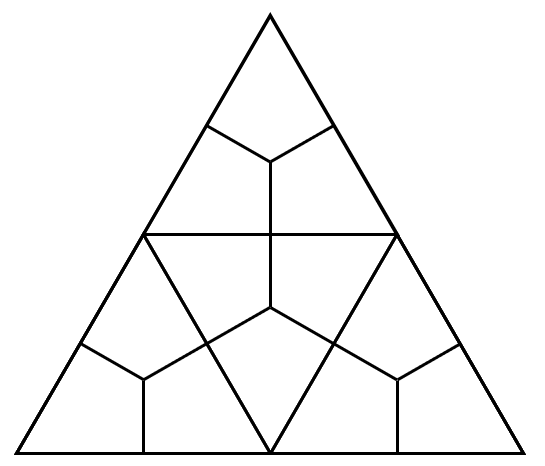
\includegraphics[width=0.5\textwidth]{Figures/Sketches/Finer_quad.png}
        \caption{4 triangles made into 12 quadrilateral elements}
    \end{subfigure}
    \hfill
    \begin{subfigure}{0.48\textwidth}
        \centering
        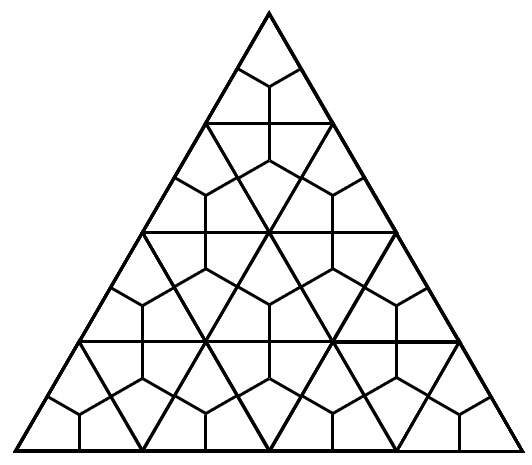
\includegraphics[width=0.5\textwidth]{Figures/Sketches/Finest_Quad.png}
        \caption{16 triangles made into 48 quadrilateral elements}
    \end{subfigure}
    \caption{Splitting different refinement levels into quads}
    \label{fig:Quads}
\end{figure}


\paragraph{Projection and merging}
The vertices are projected radially onto the sphere, $\mathbf{v}\mapsto\mathbf{v}/|\mathbf{v}|$. Since the elements are generated triangle by triangle, a vertex shared by several elements is generated several times. We merge points closer than $10^{-10}$ (using a $k$-d tree), which gives the vertex list \texttt{VX} and the element-to-vertex table \texttt{EToV}. Only the vertices are projected onto the sphere here; the curved elements between them are defined by the mapping in section \ref{sec:dg-grid}.

\begin{figure}[H]
    \centering
    \begin{subfigure}{0.48\textwidth}
        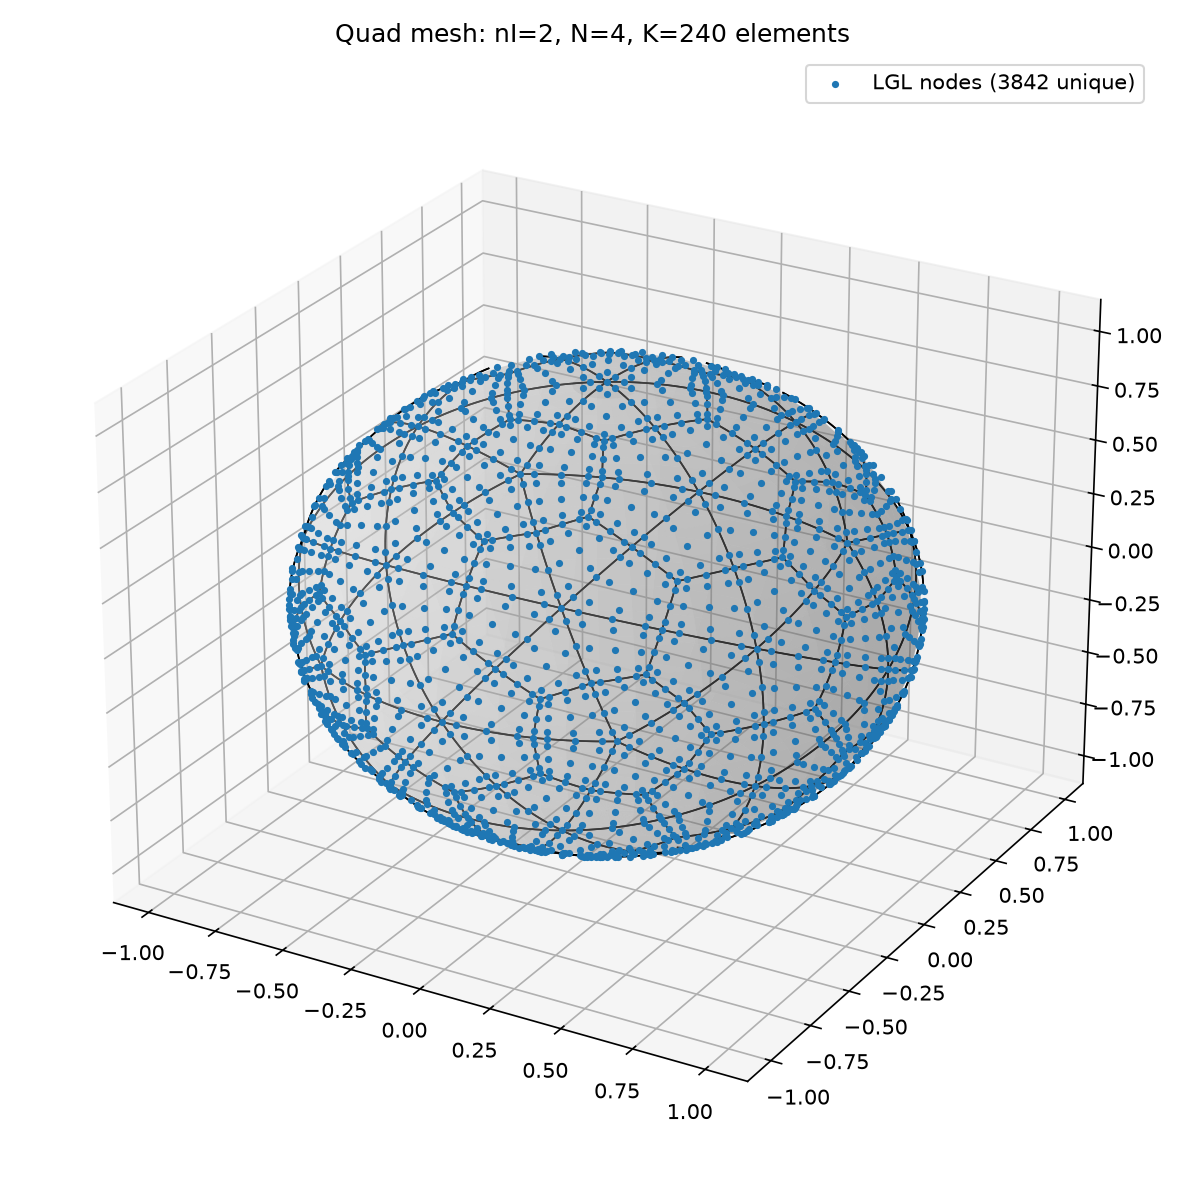
\includegraphics[width=\textwidth]{Figures/mesh_nI2_N4_K240.png}
        \caption{$n_I = 2$, $K = 240$}
    \end{subfigure}
    \hfill
    \begin{subfigure}{0.48\textwidth}
        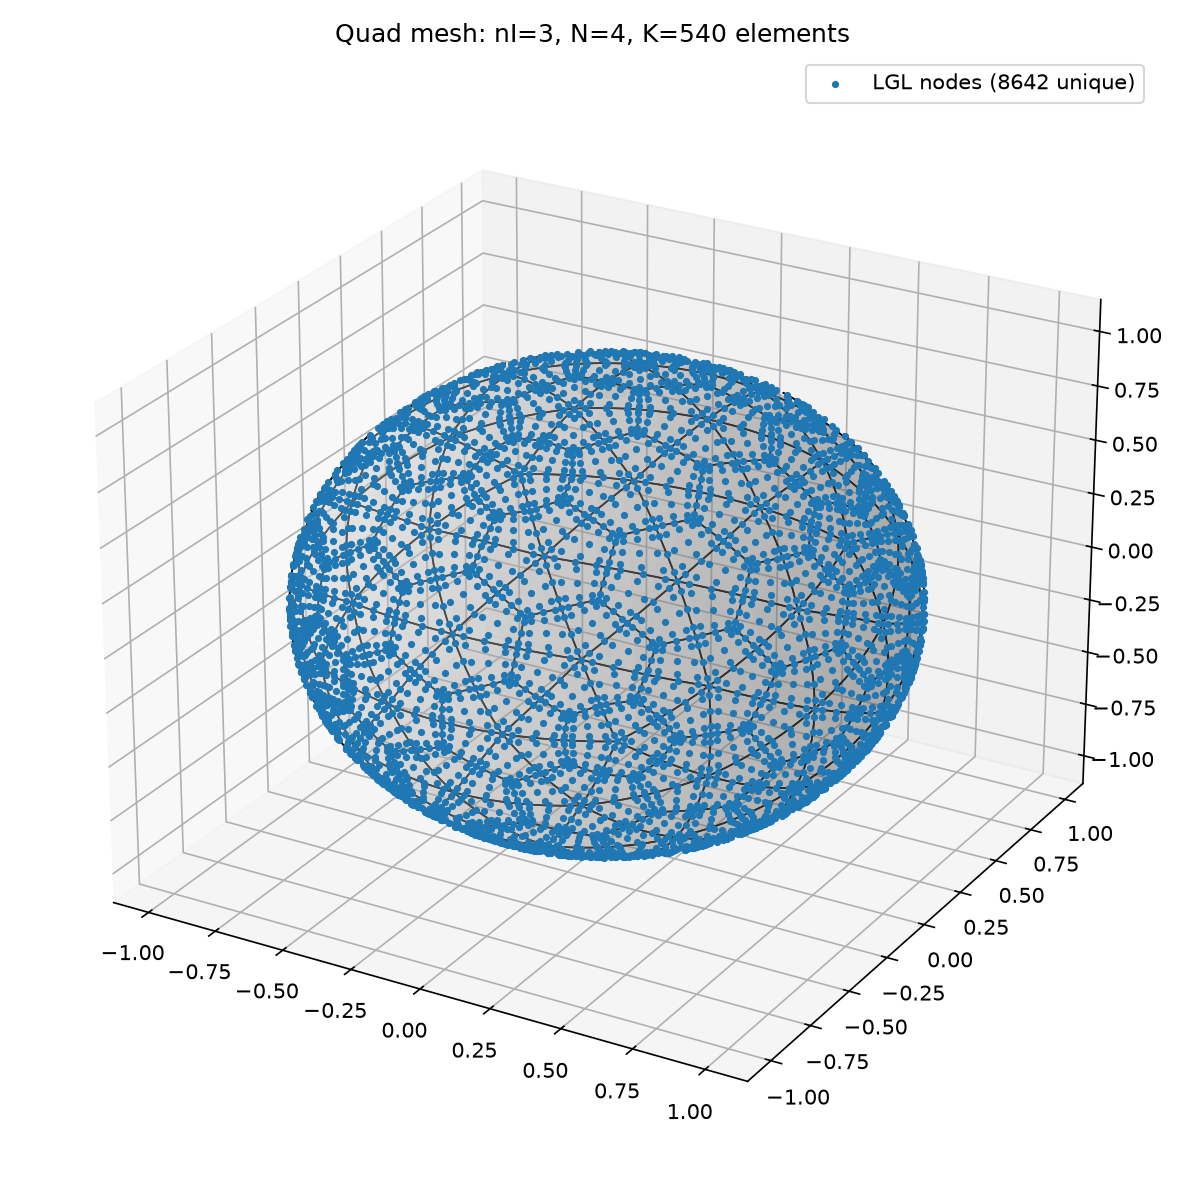
\includegraphics[width=\textwidth]{Figures/mesh_nI3_N4_K540.png}
        \caption{$n_I = 3$, $K = 540$}
    \end{subfigure}
    \caption{The icosahedral mesh with the curved elements and the LGL nodes for $N = 4$. Only the hemisphere facing the viewer is shown.}
    \label{fig:mesh}
\end{figure}

\subsection{Connectivity}\label{sec:mesh-connectivity}
The DG scheme only couples neighbouring elements through their shared sides (section \ref{sec:dg-flux}), so we need to know, for every side of every element, which element is on the other side. Side $f = 0,1,2,3$ of element $e$ runs between the local vertices $(0,1)$, $(1,2)$, $(2,3)$ and $(3,0)$. We store
\begin{itemize}
    \item \texttt{EToV}$(e,i)$: the global number of local vertex $i$ of element $e$,
    \item \texttt{EToE}$(e,f)$: the element on the other side of side $f$ of element $e$,
    \item \texttt{EToF}$(e,f)$: the local number of that side in the neighbouring element.
\end{itemize}
The tables are built in a single pass over all sides. Each side is identified by its two global vertex numbers, sorted. The first time a side is met it is stored, the second time the two elements are linked, every side is met exactly twice so every element has four neighbours and there are no boundary sides.

From \texttt{EToE} and \texttt{EToF} we build the maps from the edge nodes of each element to the edge nodes of its neighbour, which give the interior and exterior values $\mathbf{q}^-$ and $\mathbf{q}^+$ in the numerical flux. Two neighbouring elements both counter-clockwise traverse their shared side in opposite directions, the order of the edge nodes must be reversed on one side.
\section{Discretization of spherical SWEs}
We now present the discretization of the spherical SWEs. We follow \cite{GIRALDO2002499} and \cite{bonev2018discontinuous}: the equations are kept in Cartesian form, the sphere is covered by curved quadrilaterals built from an icosahedron, and on each element the solution is approximated by a tensor product of Lagrange polynomials on the Legendre--Gauss--Lobatto (LGL) points. The equations are satisfied element-wise in the strong form, the elements only communicate through a numerical flux on their edges and the constraint $\mathbf{u}\cdot\mathbf{n} = 0$ is enforced by projecting the momentum at the nodes. 


\subsection{Conservation form}\label{sec:dg-conservation}
We write the system (eq. \ref{eq:system1}, \ref{eq:system2}) in conservative form, in accordance with \cite{GIRALDO2002499}:
\begin{equation}\label{eq:conservation}
    \frac{\partial \mathbf{q}}{\partial t} + \nabla_s\cdot \mathbf{F}(\mathbf{q}) = \mathbf{S}(\mathbf{x}, \mathbf{q})
\end{equation}
where $\mathbf{q} = [h,\, hu,\, hv,\, hw]^T$, with the velocity $\mathbf{u} = (u,v,w)$ and position $\mathbf{x} = (x,y,z)$ on the sphere. The divergence $\nabla_s\cdot$ is the surface divergence, which we apply row-wise.

\paragraph{Pressure term}
In section 3 we used the projected pressure tensor $\frac12gh^2\mathbf{P}$, since the divergence theorem on the curved surface requires the rows of the flux to be tangential. In the discretization we follow \cite{GIRALDO2002499,bonev2018discontinuous} and use $\frac12gh^2\mathbf{I}$ instead. The two only differ by a normal vector: with $\nabla_s\cdot\mathbf{P} = -\frac{2}{R}\mathbf{n}$ from section 3 and $\nabla_s\cdot(\frac12gh^2\mathbf{I}) = \nabla_s(\frac12gh^2)$ we have
\begin{equation}\label{eq:dg-PvsI}
    \nabla_s\cdot\left(\tfrac12gh^2\mathbf{P}\right) = \nabla_s\cdot\left(\tfrac12gh^2\mathbf{I}\right) - \frac{gh^2}{R}\mathbf{n}.
\end{equation}
The tangential equations, which are the physical ones, are therefore the same, and the normal part $-\frac{gh^2}{R}\mathbf{n}$ is absorbed by the Lagrange multiplier. In the scheme the pressure enters in two places. On the edges it enters through $\mathbf{F}\hat{\mathbf{n}}$, where $\mathbf{P}\hat{\mathbf{n}} = \mathbf{I}\hat{\mathbf{n}} = \hat{\mathbf{n}}$, so the choice makes no difference. In the volume we evaluate the pressure gradient together with the bottom force as $gh\nabla_s(h + b)$, which is tangential (section \ref{sec:dg-forms}). The $\mathbf{I}$-form keeps the flux simple and is the form used in the literature.

\paragraph{Flux}
The rows of $\mathbf{F}$ are the mass flux $h\mathbf{u}$ followed by the rows of the momentum flux tensor
\begin{equation*}
    \mathbf{F}_m = h\mathbf{u}\otimes\mathbf{u} + \frac12 gh^2\mathbf{I}, \qquad
    (\mathbf{F}_m)_{ij} = h u_i u_j + \frac12 gh^2\delta_{ij}.
\end{equation*}
Writing $\mathbf{F}$ column-wise we get:
\begin{equation*}
    \mathbf{F} =
    \begin{bmatrix}
    hu\\
    hu^2 + \frac12 gh^2\\
    huv\\
    huw
    \end{bmatrix}\hat{\mathbf{i}} +
    \begin{bmatrix}
    hv\\
    huv\\
    hv^2 + \frac12 gh^2\\
    hvw
    \end{bmatrix}\hat{\mathbf{j}} +
    \begin{bmatrix}
    hw\\
    huw\\
    hvw\\
    hw^2 + \frac12 gh^2
    \end{bmatrix}\hat{\mathbf{k}},
\end{equation*}
which is eq. 2 of \cite{GIRALDO2002499} with the geopotential replaced by $gh$. We denote the three columns by $\mathbf{F}^{(x)}$, $\mathbf{F}^{(y)}$ and $\mathbf{F}^{(z)}$, such that $\mathbf{F} = \mathbf{F}^{(x)}\hat{\mathbf{i}} + \mathbf{F}^{(y)}\hat{\mathbf{j}} + \mathbf{F}^{(z)}\hat{\mathbf{k}}$. We also split the flux into its advective part and its pressure part,
\begin{equation}\label{eq:dg-fluxsplit}
    \mathbf{F} = \mathbf{F}^A + \mathbf{F}^p, \qquad
    \mathbf{F}^A =
    \begin{bmatrix}
    h\mathbf{u}\\
    h\mathbf{u}\otimes\mathbf{u}
    \end{bmatrix}, \qquad
    \mathbf{F}^p =
    \begin{bmatrix}
    \mathbf{0}\\
    \frac12gh^2\mathbf{I}
    \end{bmatrix},
\end{equation}
since the two parts are discretized differently in the volume (section \ref{sec:dg-operators}).

\paragraph{Source}
The source term acts only on the momentum equations \cite{GIRALDO2002499}:
\begin{equation*}
    \mathbf{S}(\mathbf{x}, \mathbf{q}) =
    \begin{bmatrix}
    0\\
    -\frac{2\omega z}{R^2}\,\mathbf{x}\times(h\mathbf{u}) - gh\nabla_s b + \lambda\mathbf{n}
    \end{bmatrix},
    \qquad
    \mathbf{x}\times(h\mathbf{u}) = h
    \begin{bmatrix}
    yw - zv\\
    zu - xw\\
    xv - yu
    \end{bmatrix}
\end{equation*}
Since $z = R\sin\phi$ and $\mathbf{n} = \mathbf{x}/R$, the Coriolis term equals $-f\mathbf{n}\times(h\mathbf{u})$ with $f = 2\omega\sin\phi$, which is purely tangential, and the bottom force $-gh\nabla_s b$ is tangential since $\nabla_s b$ is. To find $\lambda$ we take the normal component of the momentum equation. The pressure term $\nabla_s\cdot(\frac12gh^2\mathbf{I}) = gh\nabla_s h$ is tangential, and the normal part of the advective term is $\mathbf{n}\cdot\nabla_s\cdot(h\mathbf{u}\otimes\mathbf{u}) = -h|\mathbf{u}|^2/R$ (section 3.2), so
\begin{equation*}
    \lambda = -\frac{h|\mathbf{u}|^2}{R},
    \qquad
    \lambda\mathbf{n} = -\frac{h|\mathbf{u}|^2}{R^2}\,\mathbf{x}.
\end{equation*}
With $\mathbf{I}$ in the flux, the Lagrange multiplier only supplies the centripetal force. The normal pressure part $-\frac{gh^2}{R}$ from section 3 does not appear, since the divergence of the $\mathbf{I}$-flux has no normal pressure part, eq. \eqref{eq:dg-PvsI}.


\subsection{Element mapping}\label{sec:dg-grid}
\paragraph{Icosahedral grid}
We cover the sphere $S$ with $K$ non-overlapping curved quadrilaterals $\Omega^e$,
\begin{equation*}
    S = \bigcup_{e=1}^{K}\Omega^e ,
\end{equation*}
using the icosahedral grid of \cite{GIRALDO2002499}, \cite{bonev2018discontinuous}. 

Every element is mapped from the reference square $I = [-1,1]^2$ with the coordinates $\boldsymbol{\xi} = (\xi,\eta)$, see Fig.~1 in \cite{GIRALDO2002499}. Let $\mathbf{v}_1,\dots,\mathbf{v}_4$ be the vertices of $\Omega^e$, ordered counter-clockwise when seen from outside the sphere and corresponding to the reference vertices $(-1,-1)$, $(1,-1)$, $(1,1)$ and $(-1,1)$. We define the bilinear surface through the vertices
\begin{equation}
    \mathbf{X}(\xi,\eta) = \frac14\Big[(1-\xi)(1-\eta)\mathbf{v}_1 + (1+\xi)(1-\eta)\mathbf{v}_2 + (1+\xi)(1+\eta)\mathbf{v}_3 + (1-\xi)(1+\eta)\mathbf{v}_4\Big],
\end{equation}
and obtain the curved element by projecting it on the sphere:
\begin{equation}\label{eq:dg-mapping}
    \mathbf{x} = \boldsymbol{\Psi}^e(\xi,\eta) = R\frac{\mathbf{X}(\xi,\eta)}{|\mathbf{X}(\xi,\eta)|}, \qquad \mathbf{n} = \frac{\mathbf{x}}{R} = \frac{\mathbf{X}}{|\mathbf{X}|}.
\end{equation}
The mapping is exact: every point of the element lies on the sphere, and no polynomial approximation of the geometry is made. We also need a third radial reference coordinate, this corresponds to $\mathbf{x}(\xi,\eta,\rho) = \rho\,\mathbf{X}/|\mathbf{X}|$ with the surface at $\rho = R$, such that $\partial\mathbf{x}/\partial\rho = \mathbf{n}$. Functions on the sphere are extended to be constant along $\rho$, so their gradient has no normal part.

\paragraph{Jacobian}
The derivatives of the bilinear surface,
\begin{equation*}
    \mathbf{X}_\xi = \frac14\Big[(1-\eta)(\mathbf{v}_2 - \mathbf{v}_1) + (1+\eta)(\mathbf{v}_3 - \mathbf{v}_4)\Big], \qquad
    \mathbf{X}_\eta = \frac14\Big[(1-\xi)(\mathbf{v}_4 - \mathbf{v}_1) + (1+\xi)(\mathbf{v}_3 - \mathbf{v}_2)\Big],
\end{equation*}
are linear in $\eta$ and $\xi$, respectively. Differentiating the projection we get
\begin{equation*}
    \frac{\partial}{\partial\xi}\left(\frac{\mathbf{X}}{|\mathbf{X}|}\right)
    = \frac{\mathbf{X}_\xi}{|\mathbf{X}|} - \frac{\mathbf{X}(\mathbf{X}\cdot\mathbf{X}_\xi)}{|\mathbf{X}|^3}
    = \frac{1}{|\mathbf{X}|}\left(\mathbf{I} - \mathbf{n}\mathbf{n}^T\right)\mathbf{X}_\xi,
\end{equation*}
so the covariant (tangent) vectors are
\begin{equation}\label{eq:dg-covariant}
    \mathbf{x}_\xi = \frac{\partial\mathbf{x}}{\partial\xi} = \frac{R}{|\mathbf{X}|}\mathbf{P}\mathbf{X}_\xi, \qquad
    \mathbf{x}_\eta = \frac{\partial\mathbf{x}}{\partial\eta} = \frac{R}{|\mathbf{X}|}\mathbf{P}\mathbf{X}_\eta .
\end{equation}

The area element is $dA = |\mathbf{x}_\xi\times\mathbf{x}_\eta|\,d\xi\,d\eta$. Both vectors are tangential, so their cross product is parallel to $\mathbf{n}$, and we define the Jacobian
\begin{equation}
    J = \mathbf{n}\cdot(\mathbf{x}_\xi\times\mathbf{x}_\eta) = |\mathbf{x}_\xi\times\mathbf{x}_\eta|,
\end{equation}
which is positive for counter-clockwise vertices. This is the Jacobian $|J| = \frac{\partial\mathbf{x}}{\partial\zeta}\cdot\mathbf{G}$ of \cite{GIRALDO2002499} (with their radial coordinate $\zeta$) for $\partial\mathbf{x}/\partial\rho = \mathbf{n}$ and $\mathbf{G} = \mathbf{x}_\xi\times\mathbf{x}_\eta$. To write it out we use
\begin{equation*}
    \mathbf{n}\cdot(\mathbf{P}\mathbf{X}_\xi\times\mathbf{P}\mathbf{X}_\eta) = \det[\mathbf{n},\mathbf{P}\mathbf{X}_\xi,\mathbf{P}\mathbf{X}_\eta] = \det[\mathbf{n},\mathbf{X}_\xi,\mathbf{X}_\eta] = \mathbf{n}\cdot(\mathbf{X}_\xi\times\mathbf{X}_\eta),
\end{equation*}
since subtracting multiples of $\mathbf{n}$ from the last two columns does not change the determinant. With $\mathbf{n} = \mathbf{X}/|\mathbf{X}|$ the Jacobian is
\begin{equation}\label{eq:dg-jacobian}
    J^e(\xi,\eta) = \frac{R^2}{|\mathbf{X}|^2}\,\mathbf{n}\cdot(\mathbf{X}_\xi\times\mathbf{X}_\eta) = \frac{R^2}{|\mathbf{X}(\xi,\eta)|^3}\,\mathbf{X}\cdot(\mathbf{X}_\xi\times\mathbf{X}_\eta).
\end{equation}
For small elements $|\mathbf{X}|\approx R$, and $J^e$ is close to the Jacobian $|\mathbf{X}_\xi\times\mathbf{X}_\eta|$ of the bilinear surface.

To differentiate a function $f(\xi,\eta)$ on the element we need the surface gradient,
\begin{equation}\label{eq:dg-surfgrad}
    \nabla_s f = \frac{\partial f}{\partial\xi}\nabla_s\xi + \frac{\partial f}{\partial\eta}\nabla_s\eta,
\end{equation}
where the vectors $\nabla_s\xi$ and $\nabla_s\eta$ are tangential and satisfy $\nabla_s\xi\cdot\mathbf{x}_\xi = 1$, $\nabla_s\xi\cdot\mathbf{x}_\eta = 0$, $\nabla_s\eta\cdot\mathbf{x}_\xi = 0$ and $\nabla_s\eta\cdot\mathbf{x}_\eta = 1$. They are given by
\begin{equation}
    \nabla_s\xi = \frac{\mathbf{x}_\eta\times\mathbf{n}}{J}, \qquad \nabla_s\eta = \frac{\mathbf{n}\times\mathbf{x}_\xi}{J}.
\end{equation}
For example $\nabla_s\xi\cdot\mathbf{x}_\xi = (\mathbf{x}_\eta\times\mathbf{n})\cdot\mathbf{x}_\xi/J = \mathbf{n}\cdot(\mathbf{x}_\xi\times\mathbf{x}_\eta)/J = 1$, and $\nabla_s\xi\cdot\mathbf{x}_\eta = 0$ since $\mathbf{x}_\eta\times\mathbf{n}$ is perpendicular to $\mathbf{x}_\eta$. Together with $\nabla\rho = \mathbf{n}$ they are the rows of the inverse of the matrix $[\mathbf{x}_\xi,\mathbf{x}_\eta,\mathbf{n}]$, i.e.\ the metric terms $\nabla\xi$, $\nabla\eta$ of \cite{GIRALDO2002499}. Inserting eqs.~\eqref{eq:dg-covariant} and \eqref{eq:dg-jacobian}, and using $\mathbf{P}\mathbf{X}_\eta\times\mathbf{n} = \mathbf{X}_\eta\times\mathbf{n}$, we can write them out:
\begin{equation}\label{eq:dg-metric}
    J\nabla_s\xi = \frac{R}{|\mathbf{X}|^2}\,\mathbf{X}_\eta\times\mathbf{X}, \qquad
    J\nabla_s\eta = \frac{R}{|\mathbf{X}|^2}\,\mathbf{X}\times\mathbf{X}_\xi .
\end{equation}
For a vector field $\mathbf{v}$ given by its Cartesian components, such as a row of $\mathbf{F}$, the surface divergence follows by applying the surface gradient to each component:
\begin{equation}\label{eq:dg-surfdiv}
    \nabla_s\cdot\mathbf{v} = \sum_j(\nabla_s v_j)_j = \nabla_s\xi\cdot\frac{\partial\mathbf{v}}{\partial\xi} + \nabla_s\eta\cdot\frac{\partial\mathbf{v}}{\partial\eta}.
\end{equation}

\subsection{Local polynomial approximation}\label{sec:dg-poly}

\paragraph{Nodal basis}
On the reference square we use the tensor product of one-dimensional Lagrange polynomials on the $N+1$ LGL points $\xi_0,\dots,\xi_N$, which are the roots of $(1-\xi^2)P_N'(\xi)$, where $P_N$ is the Legendre polynomial of degree $N$ \cite{GIRALDO2002499}:
\begin{equation}
    L_m(\xi,\eta) = \ell_a(\xi)\,\ell_c(\eta), \qquad \ell_a(\xi_k) = \delta_{ak}, \qquad m = (a,c),\quad a,c = 0,\dots,N .
\end{equation}
Each element thus has $N_p = (N+1)^2$ nodes $\boldsymbol{\xi}_m = (\xi_a,\xi_c)$. The LGL points include $\pm1$, so each side of the element carries $N+1$ nodes, and since the points are symmetric, two neighbouring elements have the same nodes on their shared edge.

\paragraph{Local solution}
On element $\Omega^e$ the physical nodes are $\mathbf{x}^e_m = \boldsymbol{\Psi}^e(\boldsymbol{\xi}_m)$, which lie exactly on the sphere. The local solution is
\begin{equation}
    \mathbf{q}^e_N(\mathbf{x},t) = \sum_{m=1}^{N_p}\mathbf{q}^e_m(t)\,L_m(\xi,\eta), \qquad \mathbf{x} = \boldsymbol{\Psi}^e(\xi,\eta),
\end{equation}
where the nodal values $\mathbf{q}^e_m(t) = \mathbf{q}^e_N(\mathbf{x}^e_m,t)$ are the unknowns. As in \cite{GIRALDO2002499,bonev2018discontinuous}, the flux and the source are represented by their interpolants,
\begin{equation}\label{eq:dg-interp}
    \mathbf{F}_N = \sum_{m=1}^{N_p}\mathbf{F}(\mathbf{q}^e_m)\,L_m, \qquad \mathbf{S}_N = \sum_{m=1}^{N_p}\mathbf{S}(\mathbf{x}^e_m,\mathbf{q}^e_m)\,L_m,
\end{equation}
which only requires the flux and the source at the nodes.

\paragraph{Bathymetry}
The bathymetry is represented in the same way, by its values at the nodes \cite{bonev2018discontinuous}:
\begin{equation}\label{eq:dg-bathy}
    b_N = \sum_{m=1}^{N_p}b(\mathbf{x}^e_m)\,L_m .
\end{equation}
The values $b(\mathbf{x}^e_m)$ are obtained by interpolating bathymetry data, e.g.\ the ETOPO1 data set used in \cite{bonev2018discontinuous}, at the nodes. Since neighbouring elements have the same nodes on their shared edge, they get the same values there, and $b_N$ is continuous across the edges. This is used for the lake at rest in section \ref{sec:dg-forms}.

\paragraph{Integration}
The LGL points come with the quadrature weights
\begin{equation*}
    \omega_a = \frac{2}{N(N+1)}\frac{1}{P_N(\xi_a)^2},
\end{equation*}
which integrate polynomials of degree $2N-1$ exactly in one dimension. Integrals over an element and its sides are moved to the reference square with the Jacobians from section \ref{sec:dg-grid} and approximated by the tensor-product rule at the nodes,
\begin{align}
    \int_{\Omega^e}f\,dA &= \int_I f\,J^e\,d\xi\,d\eta \approx \sum_{a,c=0}^{N}\omega_a\omega_c\,f(\xi_a,\xi_c)\,J^e(\xi_a,\xi_c), \label{eq:dg-quad}\\
    \int_{\text{side 1}}f\,dS &\approx \sum_{a=0}^{N}\omega_a\,f(\xi_a,-1)\,J_s(\xi_a,-1), \nonumber
\end{align}
and likewise for the other sides. Since the quadrature points are the nodes, the quadrature is collocated, and no interpolation to other points is needed.

\paragraph{Differentiation}
Derivatives in the reference square are computed with the one-dimensional differentiation matrix $\hat{\mathcal{D}}_{ak} = \ell_k'(\xi_a)$ \cite{hesthaven2008nodal}. For nodal values $f_{ac} = f(\xi_a,\xi_c)$,
\begin{equation*}
    \left(\partial_\xi f\right)_{ac} = \sum_{k}\hat{\mathcal{D}}_{ak}f_{kc}, \qquad \left(\partial_\eta f\right)_{ac} = \sum_{k}\hat{\mathcal{D}}_{ck}f_{ak},
\end{equation*}
i.e.\ the one-dimensional matrix is applied along each line of nodes. This costs $\mathcal{O}(N^3)$ operations per element instead of $\mathcal{O}(N^4)$ for a full two-dimensional matrix. Together with eqs.~\eqref{eq:dg-surfgrad} and \eqref{eq:dg-surfdiv} this gives the surface gradient and divergence at the nodes.

\paragraph{Summation by parts}
For two polynomials $f$ and $g$ of degree $N$, $f'g + fg'$ has degree $2N-1$, so the LGL rule integrates it exactly and
\begin{equation}\label{eq:dg-sbp}
    \sum_{a=0}^{N}\omega_a\,(\hat{\mathcal{D}}f)_a\,g_a + \sum_{a=0}^{N}\omega_a\,f_a\,(\hat{\mathcal{D}}g)_a = f(1)g(1) - f(-1)g(-1).
\end{equation}
This discrete integration by parts holds exactly for any nodal values, and it relates the strong and the weak forms in section \ref{sec:dg-forms}.

\paragraph{Exact and inexact integration}
Counting the degrees in each reference coordinate:
\begin{itemize}
    \item The mass matrix, $\int L_lL_m\,dA$, has the polynomial part $L_lL_m$ of degree $2N$, multiplied by $J^e$. The LGL rule is therefore not exact even on a flat element. It makes the mass matrix diagonal (section \ref{sec:dg-operators}).
    \item The divergence term, $\int L_l\nabla_s L_m\,dA$, has the polynomial part of degree $2N-1$, multiplied by $J\nabla_s\xi$ and $J\nabla_s\eta$ from eq.~\eqref{eq:dg-metric}.
    \item The flux is nonlinear in $\mathbf{q}_N$: $\frac12gh^2$ has degree $2N$, and $h\mathbf{u}\otimes\mathbf{u} = (h\mathbf{u})\otimes(h\mathbf{u})/h$ is a rational function. The bottom force $gh\nabla_s b$ has degree $2N-1$.
    \item The Coriolis term contains the product of $z$, $\mathbf{x}$ and $h\mathbf{u}$, which together with the test function gives the highest degree, $4N$, cf.\ the Coriolis matrix of \cite{GIRALDO2002499}.
\end{itemize}
Using the LGL rule at the nodes is what \cite{GIRALDO2002499} call inexact integration. It is equivalent to replacing each integrand by its interpolant at the nodes, i.e.\ to using $\mathbf{F}_N$ and $\mathbf{S}_N$ from eq.~\eqref{eq:dg-interp}. Exact integration (over-integration) instead interpolates the solution to $Q > N+1$ Gauss points per direction, evaluates the flux and the source there and integrates with Gauss quadrature. For the Coriolis term \cite{GIRALDO2002499} give $Q = (cN+1)/2$ with $c = 4$. This costs about $(Q/(N+1))^2$ times as many flux evaluations in every evaluation of the right hand side, and it still cannot integrate the rational geometric factors exactly. \cite{GIRALDO2002499} found the strong form to be robust to inexact integration and diagonal mass matrices (Figs.~4--5 there), and both \cite{GIRALDO2002499} and \cite{bonev2018discontinuous} use inexact integration.


\subsection{Weak and strong forms}\label{sec:dg-forms}
Using the conservative system derived in sec. \ref{sec:dg-conservation}, we now formulate the scheme on one element. We replace $\mathbf{q}$ by $\mathbf{q}_N$, multiply eq. \eqref{eq:conservation} by a test function $L_k$, $k = 1,\dots,N_p$, and integrate over $\Omega^e$. For each of the four rows of the system:
\begin{equation}\label{eq:dg-galerkin}
    \int_{\Omega^e}\left(\frac{\partial\mathbf{q}_N}{\partial t} + \nabla_s\cdot\mathbf{F}_N - \mathbf{S}_N\right)L_k\,dA = 0.
\end{equation}
This equation does not connect the elements. The solution is discontinuous between elements, so on each edge there is one value from $\Omega^e$ and one from its neighbour, and we let information pass between the elements through a single-valued numerical flux $\mathbf{F}^*\hat{\mathbf{n}}$ (section \ref{sec:dg-flux}). Taking the difference between the local and the numerical flux on the boundary gives the strong form \cite{GIRALDO2002499}:
\begin{equation}\label{eq:dg-strong}
    \int_{\Omega^e}\left(\frac{\partial\mathbf{q}_N}{\partial t} + \nabla_s\cdot\mathbf{F}_N - \mathbf{S}_N\right)L_k\,dA = \oint_{\partial\Omega^e}L_k\left(\mathbf{F}_N - \mathbf{F}^*\right)\hat{\mathbf{n}}\,dS.
\end{equation}

\paragraph{Weak form}
The weak form, is obtained by integrating the LHS by parts. For this we need the surface divergence theorem from section 3.1 for a vector field $\mathbf{v}$:
\begin{equation}\label{eq:dg-divthm}
    \int_{\Omega^e}\nabla_s\cdot\mathbf{v}\,dA = \oint_{\partial\Omega^e}\mathbf{v}\cdot\hat{\mathbf{n}}\,dS + \int_{\Omega^e}H\,\mathbf{v}\cdot\mathbf{n}\,dA, \qquad H = \frac{2}{R}.
\end{equation}
Let $\mathbf{r}_i$ be row $i$ of $\mathbf{F}_N$. We let $\mathbf{v} = L_k\mathbf{r}_i$ and use the product rule $\nabla_s\cdot(L_k\mathbf{r}_i) = L_k\nabla_s\cdot\mathbf{r}_i + \mathbf{r}_i\cdot\nabla_s L_k$:
\begin{equation}\label{eq:dg-ibp}
    \int_{\Omega^e}L_k\,\nabla_s\cdot\mathbf{r}_i\,dA = \oint_{\partial\Omega^e}L_k\,\mathbf{r}_i\cdot\hat{\mathbf{n}}\,dS - \int_{\Omega^e}\mathbf{r}_i\cdot\nabla_s L_k\,dA + \int_{\Omega^e}H L_k\,\mathbf{r}_i\cdot\mathbf{n}\,dA.
\end{equation}
Inserting this in eq.~\eqref{eq:dg-strong}, with $(\mathbf{F}\mathbf{v})_i = \mathbf{r}_i\cdot\mathbf{v}$ as in sec. 3, gives
\begin{equation}\label{eq:dg-weak}
    \int_{\Omega^e}\frac{\partial\mathbf{q}_N}{\partial t}L_k\,dA - \int_{\Omega^e}\mathbf{F}_N\nabla_s L_k\,dA + \int_{\Omega^e}H L_k\,\mathbf{F}_N\mathbf{n}\,dA = \int_{\Omega^e}\mathbf{S}_N L_k\,dA - \oint_{\partial\Omega^e}L_k\,\mathbf{F}^*\hat{\mathbf{n}}\,dS.
\end{equation}
The third term is the curvature term. With $\frac12gh^2\mathbf{I}$ the momentum rows are not tangential, $(\mathbf{F}\mathbf{n})_i = hu_i(\mathbf{u}\cdot\mathbf{n}) + \frac12gh^2n_i = \frac12gh^2n_i$, so in the weak form the curvature term must be kept. The strong form contains no curvature term at all, which is one reason to use it together with $\mathbf{I}$. With $\mathbf{P}$, as in sec. 3, the curvature term would vanish in the weak form instead.

\paragraph{Lake at rest}
Following \cite{bonev2018discontinuous} (Propositions 1 and 2), the strong form preserves a steady state exactly if $\nabla_s\cdot\mathbf{F}_N - \mathbf{S}_N = 0$ at the nodes and $\mathbf{F}^* = \mathbf{F}_N$ on the edges, since then both integrands in eq.~\eqref{eq:dg-strong} vanish. The steady state is the lake at rest from section \ref{sec:sph-rest}, $\mathbf{u} = 0$ and $h + b = \zeta_0$. For $\mathbf{u} = 0$ the advective flux and the Coriolis force vanish, and the tangential part of the momentum rows of $\nabla_s\cdot\mathbf{F} - \mathbf{S}$ is
\begin{equation*}
    \nabla_s\left(\tfrac12gh^2\right) + gh\nabla_s b = gh\nabla_s(h + b) .
\end{equation*}
In the continuous problem the two terms on the LHS cancel. If we discretize them separately, the first as the derivative of the interpolant of $\frac12gh^2$ and the second with $b_N$, they do not cancel at the nodes, since the discrete derivative does not satisfy the product rule, $\nabla_s\mathcal{I}_N(\frac12gh^2)\neq gh\nabla_s h_N$. What is left is a false force which, even with a small relative error, can produce false waves (section \ref{sec:sph-rest}). Following \cite{bonev2018discontinuous}, we evaluate the pressure gradient and the bottom force together at the nodes, as
\begin{equation}\label{eq:dg-pressurebottom}
    g h_k\left(\nabla_s\zeta_N\right)_k, \qquad \zeta_N = h_N + b_N .
\end{equation}
For the lake at rest $\zeta_N$ is $\zeta_0$ at every node, so
\begin{equation*}
    \nabla_s\zeta_N = \sum_k\zeta_0\nabla_s L_k = \zeta_0\nabla_s\Big(\sum_k L_k\Big) = 0
\end{equation*}
since the Lagrange polynomials sum to one. On the edges, $b_N$ and $h_N = \zeta_0 - b_N$ is continuous (section \ref{sec:dg-poly}), so the numerical flux and the local flux are consistent, $\mathbf{F}^* = \mathbf{F}_N$. The lake at rest is therefore preserved. For a flat bottom it reduces to the fluid at rest. 

Because we use a conforming grid we do not need to modify the numerical flux as in \cite{bonev2018discontinuous} (eqs. 43-45 there). However the dry nodes do require a modification of eq. \eqref{eq:dg-pressurebottom} (see sec. \ref{sec:dg-wetdry})

\paragraph{Mass conservation}
In the weak form we sum eq.~\eqref{eq:dg-weak} over $k$ for the first row and use $\sum_k L_k = 1$. The volume term vanishes since $\sum_k\nabla_s L_k = 0$, and the curvature term of the mass row vanishes at the nodes where $(h\mathbf{u})\cdot\mathbf{n} = 0$. This leaves
\begin{equation*}
    \frac{d}{dt}\int_{\Omega^e}h_N\,dA = -\oint_{\partial\Omega^e}\left(\mathbf{F}^*\hat{\mathbf{n}}\right)_1 dS .
\end{equation*}
The change of mass in an element equals the flux through its edges, as in sec. \ref{sec:car-Mass}. If we sum over all elements every edge appears twice with opposite normals $\hat{\mathbf{n}}^+ = -\hat{\mathbf{n}}^-$ and the numerical flux changes sign with the normal (section \ref{sec:dg-flux}), so the edge contributions cancel and the weak form conserves the total mass exactly.

In the strong form the same sum gives
\begin{equation*}
    \frac{d}{dt}\int_{\Omega^e}h_N\,dA = -\int_{\Omega^e}\nabla_s\cdot(h\mathbf{u})_N\,dA + \oint_{\partial\Omega^e}(h\mathbf{u})_N\cdot\hat{\mathbf{n}}\,dS - \oint_{\partial\Omega^e}\left(\mathbf{F}^*\hat{\mathbf{n}}\right)_1 dS,
\end{equation*}
so mass is conserved exactly if the first two terms cancel. Applying the summation by parts eq.~\eqref{eq:dg-sbp} in both directions to eq.~\eqref{eq:dg-surfdiv} shows that the two terms differ by
\begin{equation*}
    \sum_{a,c}\omega_a\omega_c\,J\,(h\mathbf{u})\cdot\frac{1}{J}\left[\hat\partial_\xi\left(J\nabla_s\xi\right) + \hat\partial_\eta\left(J\nabla_s\eta\right)\right]_{ac},
\end{equation*}
where $\hat\partial_\xi$, $\hat\partial_\eta$ are the discrete derivatives. Since $(h\mathbf{u})\cdot\mathbf{n} = 0$ at the nodes, this is exactly the tangential error of the discrete metric identity, eq.~\eqref{eq:dg-metricid}. The same error decides whether the weak form preserves the lake at rest: if the discrete metric identity holds, the two forms are identical and have both properties; the role of the metric identities in the two forms is analysed in \cite{kopriva2006metric}. 

On the sphere the discrete metric identity only holds up to the interpolation error of the metric terms. The strong form therefore conserves mass with an error that decreases spectrally with $N$, while the weak form preserves the lake at rest only to the same accuracy. Following \cite{bonev2018discontinuous} we want the exact preservation of the steady state, using the strong form and we monitor the total mass as a diagnostic.

\subsection{Numerical flux}\label{sec:dg-flux}
At an edge node we denote the value from the element itself by $\mathbf{q}^-$ and the value from the neighbour by $\mathbf{q}^+$, and $\hat{\mathbf{n}}$ is the outward normal of the element. Since both elements use the same Cartesian components, $\mathbf{q}^+$ can be used directly, without rotating the momentum into a local coordinate system.

With $\mathbf{I}\hat{\mathbf{n}} = \hat{\mathbf{n}}$ and the normal velocity $U = \mathbf{u}\cdot\hat{\mathbf{n}}$, the normal flux is
\begin{equation}\label{eq:dg-normalflux}
    \mathbf{F}\hat{\mathbf{n}} =
    \begin{bmatrix}
    hU\\
    h\mathbf{u}\,U + \frac12gh^2\hat{\mathbf{n}}
    \end{bmatrix}.
\end{equation}
We use the Lax--Friedrichs flux as in \cite{GIRALDO2002499,bonev2018discontinuous},
\begin{equation}\label{eq:dg-lf}
    \mathbf{F}^*\hat{\mathbf{n}} = \frac12\left(\mathbf{F}(\mathbf{q}^-) + \mathbf{F}(\mathbf{q}^+)\right)\hat{\mathbf{n}} - \frac{\alpha}{2}\left(\mathbf{q}^+ - \mathbf{q}^-\right),
\end{equation}
where $\alpha$ is the largest wave speed, normal to the edge. We write $\alpha$ instead of $|\lambda|$ from \cite{GIRALDO2002499}, since $\lambda$ is the Lagrange multiplier. Seen from the neighbour, $\hat{\mathbf{n}}$ changes sign and $\mathbf{q}^-$ and $\mathbf{q}^+$ swap, which changes the sign of $\mathbf{F}^*\hat{\mathbf{n}}$. What leaves one element enters another. At dry nodes the velocity is zero (section \ref{sec:dg-wetdry}), so there $U = 0$.

\paragraph{Flux Jacobian}
To find $\alpha$ we need the eigenvalues of the flux Jacobian $\mathbf{A} = \partial(\mathbf{F}\hat{\mathbf{n}})/\partial\mathbf{q}$. We write eq.~\eqref{eq:dg-normalflux} in the conserved variables $h$ and $\mathbf{m} = h\mathbf{u}$:
\begin{equation*}
    \mathbf{F}\hat{\mathbf{n}} =
    \begin{bmatrix}
    \mathbf{m}\cdot\hat{\mathbf{n}}\\
    \frac1h\mathbf{m}(\mathbf{m}\cdot\hat{\mathbf{n}}) + \frac12gh^2\hat{\mathbf{n}}
    \end{bmatrix}.
\end{equation*}
The mass row gives $\partial(\mathbf{m}\cdot\hat{\mathbf{n}})/\partial h = 0$ and $\partial(\mathbf{m}\cdot\hat{\mathbf{n}})/\partial m_j = \hat{n}_j$. Differentiating the momentum rows gives
\begin{equation*}
    \frac{\partial}{\partial h}\left(\frac{m_i(\mathbf{m}\cdot\hat{\mathbf{n}})}{h} + \frac12gh^2\hat{n}_i\right) = -u_iU + gh\,\hat{n}_i, \qquad
    \frac{\partial}{\partial m_j}\left(\frac{m_i(\mathbf{m}\cdot\hat{\mathbf{n}})}{h}\right) = \delta_{ij}U + u_i\hat{n}_j,
\end{equation*}
so
\begin{equation}
    \mathbf{A} =
    \begin{bmatrix}
    0 & \hat{\mathbf{n}}^T\\
    gh\,\hat{\mathbf{n}} - U\mathbf{u} & U\mathbf{I} + \mathbf{u}\hat{\mathbf{n}}^T
    \end{bmatrix},
\end{equation}
which is exactly the Jacobian of \cite{GIRALDO2002499}. Since eigenvalues do not depend on the orientation of the axes we choose the axes such that $\hat{\mathbf{n}} = (1,0,0)$, the second axis is along the edge and the third along $\mathbf{n}$. Then $U = u$ and
\begin{equation*}
    \mathbf{A} =
    \begin{bmatrix}
    0 & 1 & 0 & 0\\
    gh - u^2 & 2u & 0 & 0\\
    -uv & v & u & 0\\
    -uw & w & 0 & u
    \end{bmatrix}.
\end{equation*}
The matrix is block lower triangular. The lower block gives the eigenvalue $U$ twice, and the upper block gives $\kappa^2 - 2U\kappa - (gh - U^2) = 0$, i.e.\ $\kappa = U\pm\sqrt{gh}$. The eigenvalues are thus
\begin{equation*}
    U, \quad U, \quad U + \sqrt{gh}, \quad U - \sqrt{gh},
\end{equation*}
and the largest wave speed is
\begin{equation}
    \alpha = \max\left(|U^-| + \sqrt{gh^-},\ |U^+| + \sqrt{gh^+}\right),
\end{equation}
as in eq.~22 of \cite{bonev2018discontinuous}. The eigenvalues $U\pm\sqrt{gh}$ are the waves whose speed depends on the local depth (section \ref{sec:sph-rest}). One eigenvalue $U$ moves the momentum along the edge. The other moves the normal momentum $\mathbf{m}\cdot\mathbf{n}$, a component that only exists because we use three momentum components for a two-dimensional flow, we set this to zero by constraint (section \ref{sec:dg-operators}).

The Lax--Friedrichs flux is dissipative, but the dissipation is proportional to the jump $\mathbf{q}^+ - \mathbf{q}^-$, which for a smooth solution decreases at the same rate as the approximation error. Other fluxes can be used and should be investigated in future work.

% ---------------------------------------------------------------------
\subsection{Discrete operators and semi-discrete system}\label{sec:dg-operators}
As in \cite{GIRALDO2002499} we define the mass matrix, the derivative matrices and the edge matrices,
\begin{equation*}
    \mathbf{M}^e_{lm} = \int_{\Omega^e}L_lL_m\,dA, \qquad
    (\mathbf{D}^e_j)_{lm} = \int_{\Omega^e}L_l\,(\nabla_s L_m)_j\,dA, \qquad
    \mathbf{E}^{e,f}_{lm} = \int_{\text{side } f}L_lL_m\,dS,
\end{equation*}
with one derivative matrix for each Cartesian direction, $j\in\{x,y,z\}$, and evaluate them with the LGL rule eq.~\eqref{eq:dg-quad}. Since $L_m(\boldsymbol{\xi}_l) = \delta_{lm}$:
\begin{equation}
    \mathbf{M}^e = \mathrm{diag}\left(\omega_a\omega_c\,J^e_{ac}\right), \qquad
    \mathbf{D}^e_j = \mathbf{M}^e\boldsymbol{\nabla}_j, \qquad
    \mathbf{E}^{e,1} = \mathrm{diag}\left(\omega_a\,J_s(\xi_a,-1)\right),
\end{equation}
where $\mathbf{E}^{e,1}$ acts on the nodes of side 1 (likewise for the other sides), and $(\boldsymbol{\nabla}_j)_{lm} = (\nabla_s L_m)_j(\boldsymbol{\xi}_l)$ is the derivative in the Cartesian direction $j$ at the nodes, computed with $\hat{\mathcal{D}}$ and the metric terms. The mass matrix is diagonal, which is the advantage of the quadrilateral LGL elements.

\paragraph{Semi-discrete system}
Inserting the operators in eq.~\eqref{eq:dg-strong} and dividing by the diagonal mass matrix node by node gives the semi-discrete strong form at the nodes. On side 1 the edge term at the node $(a,0)$ is divided by $\omega_a\omega_0J^e$, which leaves the factor $J_s/(\omega_0J^e)$, and likewise on the other sides. With the volume term written as discussed in section \ref{sec:dg-forms}, the system at node $m$ of element $e$ is
\begin{equation}\label{eq:dg-semistrong}
    \frac{d\mathbf{q}_m}{dt} = -\mathbf{V}_m + \mathbf{C}_m + \sum_{f=1}^{4}\frac{J_s}{\omega_0J^e}\left[\mathbf{F}_N\hat{\mathbf{n}} - \mathbf{F}^*\hat{\mathbf{n}}\right]_{m,f},
\end{equation}
with the volume term and the Coriolis term
\begin{equation}\label{eq:dg-volume}
    \mathbf{V}_m =
    \begin{bmatrix}
    \nabla_s\cdot(h\mathbf{u})_N\\
    \nabla_s\cdot(h\mathbf{u}\otimes\mathbf{u})_N + g h\,\nabla_s\zeta_N
    \end{bmatrix}_m, \qquad
    \mathbf{C}_m =
    \begin{bmatrix}
    0\\
    -\frac{2\omega z_m}{R^2}\,\mathbf{x}_m\times(h\mathbf{u})_m
    \end{bmatrix}.
\end{equation}

\paragraph{Lagrange multiplier}
We do not compute the Lagrange multiplier from the analytic expression in section \ref{sec:dg-conservation}, since the discrete right hand side does not satisfy the identities it was derived from (section \ref{sec:dg-poly}). Instead, as in \cite{GIRALDO2002499,bonev2018discontinuous}, we require that the discrete momentum stays tangential at every node. Let $\mathbf{R}_m\in\mathbb{R}^3$ be the momentum part of eq.~\eqref{eq:dg-semistrong} at node $m$, computed without $\lambda$. Requiring $\mathbf{n}_m\cdot d(h\mathbf{u})_m/dt = 0$ with $d(h\mathbf{u})_m/dt = \mathbf{R}_m + \lambda_m\mathbf{n}_m$ gives
\begin{equation}\label{eq:dg-projection}
    \lambda_m = -\mathbf{n}_m\cdot\mathbf{R}_m, \qquad \frac{d(h\mathbf{u})_m}{dt} = \mathbf{P}_m\mathbf{R}_m,
\end{equation}
with $\mathbf{P}_m = \mathbf{I} - \mathbf{n}_m\mathbf{n}_m^T$. The Lagrange multiplier is  projecting the momentum right hand side onto the tangent plane at each node. Since the mass matrix is diagonal, it makes no difference whether the projection is applied before or after dividing by it, and it is equivalent to the term $\mu\,\mathbf{I}_3\otimes\mathbf{M}$ of \cite{GIRALDO2002499}, with $\lambda = \mu R$ since $\lambda\mathbf{n} = \mu\mathbf{x}$. The initial momentum is projected in the same way. The analytic $\lambda = -h|\mathbf{u}|^2/R$ is still useful as a check: $-\mathbf{n}_m\cdot\mathbf{R}_m$ should converge to it as $N$ is increased.

\paragraph{Summary}
The semi-discrete system on each element is $d\mathbf{q}^e/dt = \mathbf{B}^e(\mathbf{q})$, where $\mathbf{B}^e$ only depends on the nodal values of the element itself and the edge values of its four neighbours. One evaluation of $\mathbf{B}^e$ consists of:
\begin{enumerate}
    \item compute the velocity $\mathbf{u} = (h\mathbf{u})/h$ at the wet nodes and set $\mathbf{u} = 0$ at the dry nodes (section \ref{sec:dg-wetdry})
    \item compute the columns of the advective flux $\mathbf{F}^A$, the free surface $\zeta = h + b$ and the Coriolis term at the nodes
    \item compute the volume term eq.~\eqref{eq:dg-volume}, using the finite-difference gradient of section \ref{sec:dg-wetdry} for $\zeta$ in semi-dry elements
    \item at the edge nodes, compute $\mathbf{F}_N\hat{\mathbf{n}}$ and the numerical flux eq.~\eqref{eq:dg-lf} from $\mathbf{q}^-$ and $\mathbf{q}^+$, and add the edge terms of eq.~\eqref{eq:dg-semistrong}
    \item project the momentum at every node with eq.~\eqref{eq:dg-projection}.
\end{enumerate}

% ---------------------------------------------------------------------
\subsection{Time integration and stabilisation}\label{sec:dg-time}

\paragraph{Runge--Kutta}
The semi-discrete system $d\mathbf{q}/dt = \mathbf{B}(\mathbf{q})$ is explicit. With dry regions we need the strong stability preserving property of section \ref{sec:dg-wetdry}, so we follow \cite{bonev2018discontinuous} and use the third-order method SSPRK(3,3):
\begin{align*}
    \mathbf{q}^{(1)} &= \mathbf{q}^n + \Delta t\,\mathbf{B}\big(\mathbf{q}^n\big),\\
    \mathbf{q}^{(2)} &= \frac34\mathbf{q}^n + \frac14\left(\mathbf{q}^{(1)} + \Delta t\,\mathbf{B}\big(\mathbf{q}^{(1)}\big)\right),\\
    \mathbf{q}^{n+1} &= \frac13\mathbf{q}^n + \frac23\left(\mathbf{q}^{(2)} + \Delta t\,\mathbf{B}\big(\mathbf{q}^{(2)}\big)\right).
\end{align*}
Each stage is a combination of the previous solution and a forward Euler step, so the positivity of the averages is kept under eq.~\eqref{eq:dg-positivity}, and we apply the positivity limiter after each stage. We use the third-order method and not the fourth-order method of \cite{GIRALDO2002499} even though the fourth-order method has a larger stability interval. The third-order method is used because it is strong stability preserving, which we need.

\paragraph{Time step}
As in \cite{GIRALDO2002499} (eq.~11 there, with the geopotential replaced by $gh$) we choose the time step as
\begin{equation}
    \Delta t \leq C_{\mathrm{CFL}}\,\min_{\text{nodes}}\left[\,|\mathbf{u}\cdot\boldsymbol{\chi}| + \sqrt{gh}\,|\boldsymbol{\chi}|\,\right]^{-1}, \qquad
    \chi_j = \frac{|(\nabla_s\xi)_j|}{\Delta\xi} + \frac{|(\nabla_s\eta)_j|}{\Delta\eta},
\end{equation}
where $\Delta\xi$ and $\Delta\eta$ are the local spacings of the LGL points in the reference square, which are smallest near the edges, where they scale like $1/N^2$, and $C_{\mathrm{CFL}}$ is of order one. The ratio $|\nabla_s\xi|/\Delta\xi$ is the inverse of the physical distance between neighbouring lines of nodes $\xi = \mathrm{const}$, so $\boldsymbol{\chi}$ measures how densely the nodes are packed in each Cartesian direction. A skewed element, such as the $60^\circ$/$120^\circ$ quadrilaterals of the icosahedral grid, could have many nodes in one direction, but not as many in others. The gravity wave speed $\sqrt{gh}$ is largest over the deepest parts of the ocean, about $310$ m/s over a depth of $10$ km, while $|\mathbf{u}|\ll\sqrt{gh}$ for tsunamis, so the time step is set by the deep-ocean gravity waves in the smallest elements.

\paragraph{Post-processing}
Collecting the above: after every stage of the Runge--Kutta method we apply the positivity limiter, set $h\mathbf{u} = 0$ at the dry nodes and project the momentum at every node. After the last stage of each time step, before these steps, the semi-dry elements are filtered on the free surface.

\section{Results}

\subsection{Verification of the geometry}\label{sec:mesh-verification}
The mesh and the mapping of section \ref{sec:dg-grid} are verified by integrating a smooth function over the sphere, for which the exact integral is known,
\begin{equation*}
    \int_S e^{\mathbf{a}\cdot\mathbf{n}}\,dA = 2\pi R^2\left(e - e^{-1}\right), \qquad |\mathbf{a}| = 1 .
\end{equation*}
This tests the vertices, the mapping, the Jacobian and the quadrature together. Figure \ref{fig:mesh-convergence} shows the relative error under $h$-refinement (increasing $n_I$) and $p$-refinement (increasing $N$). The total area of the elements also equals $4\pi R^2$ to within the quadrature error ($\approx 4\cdot10^{-7}$ relative for $n_I = 1$, $N = 4$, and below $10^{-8}$ for $n_I\geq2$), which confirms that the elements cover the sphere without gaps or overlaps.

\begin{figure}[H]
    \centering
    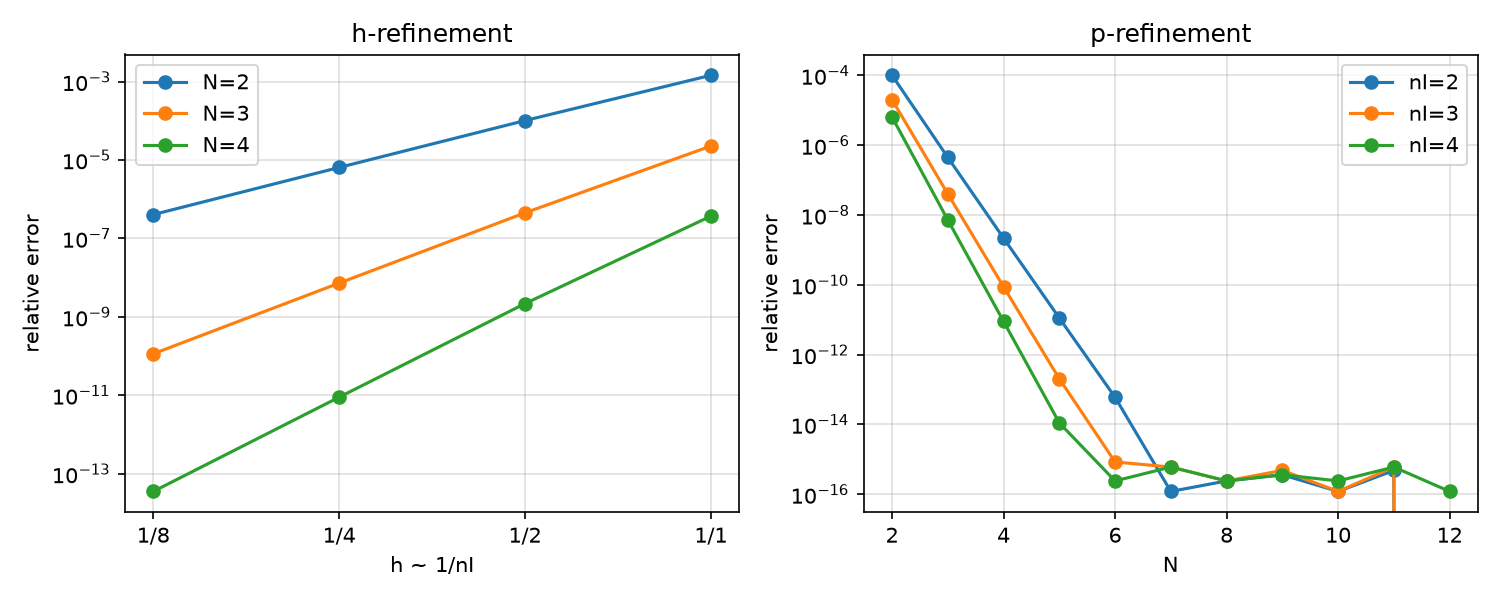
\includegraphics[width=0.9\textwidth]{Figures/convergence_integrals.png}
    \caption{Relative error of the integral of $e^{\mathbf{a}\cdot\mathbf{n}}$ over the sphere under $h$-refinement (left) and $p$-refinement (right).}
    \label{fig:mesh-convergence}
\end{figure}



\begin{figure}
    \centering
    \begin{subfigure}[t]{0.49\linewidth}
        \centering
        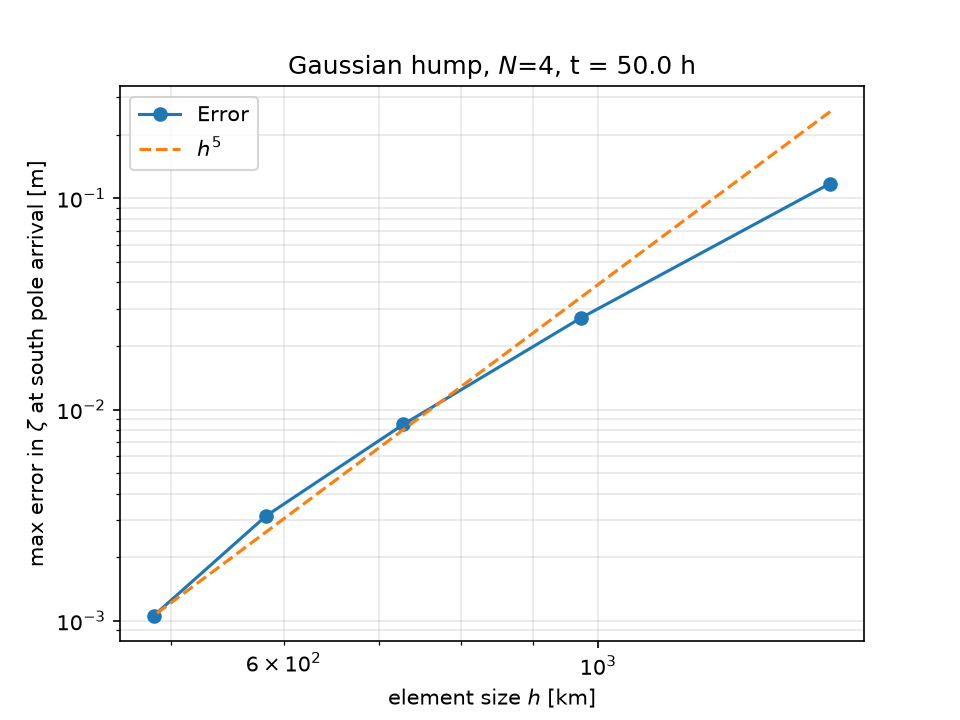
\includegraphics[width=\linewidth]{Figures/gaussian_hump_Hconvergence.png}
        \caption{h-convergence with $N=4$.}
        \label{fig:Hconvergence}
    \end{subfigure}
    \hfill
    \begin{subfigure}[t]{0.49\linewidth}
        \centering
        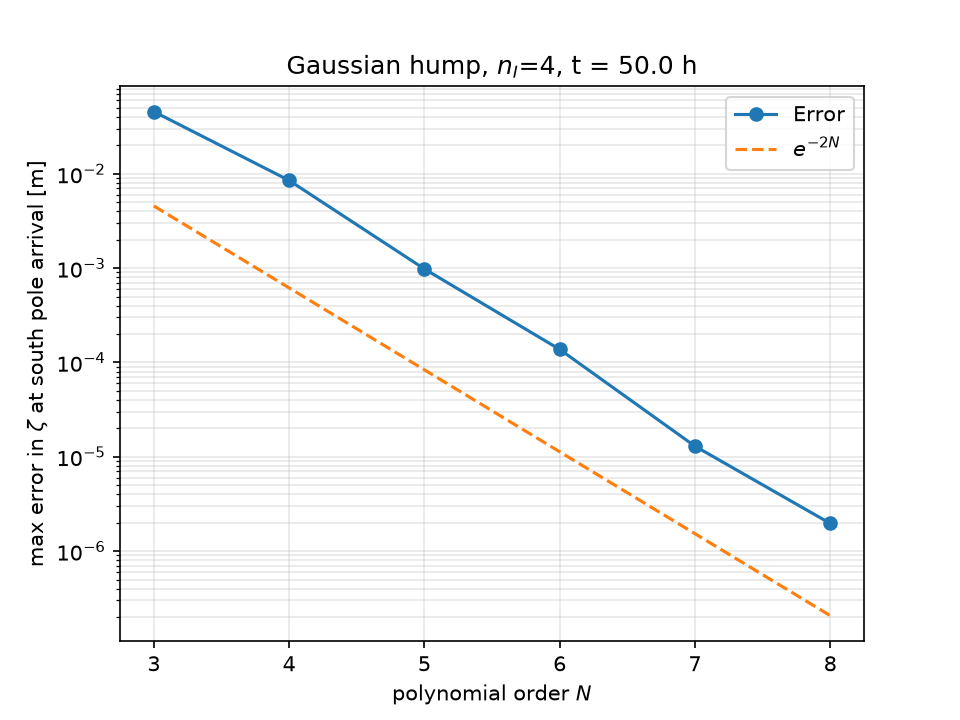
\includegraphics[width=\linewidth]{Figures/gaussian_hump_Pconvergence.png}
        \caption{p-convergence with $n_I=4$.}
        \label{fig:Pconvergence}
    \end{subfigure}
    \caption{Convergence for the Gaussian hump on the sphere. Linearized SWEs at time $t=50.0h$.}
    \label{fig:convergence}
\end{figure}

\begin{figure}
    \centering
    \begin{subfigure}[t]{0.32\linewidth}
        \centering
        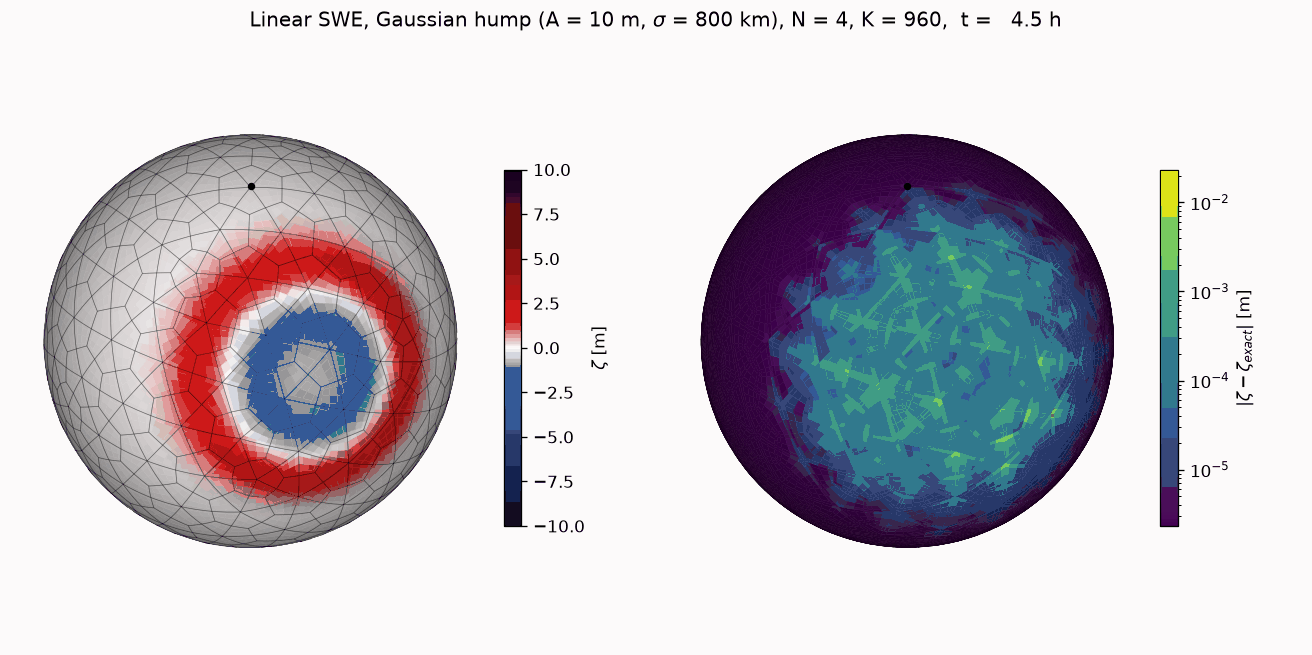
\includegraphics[width=\linewidth]{Figures/GIF_4-5h.png}
        \caption{Snapshot at 4.5h}
        \label{fig:snap4-5}
    \end{subfigure}
    \hfill
    \begin{subfigure}[t]{0.32\linewidth}
        \centering
        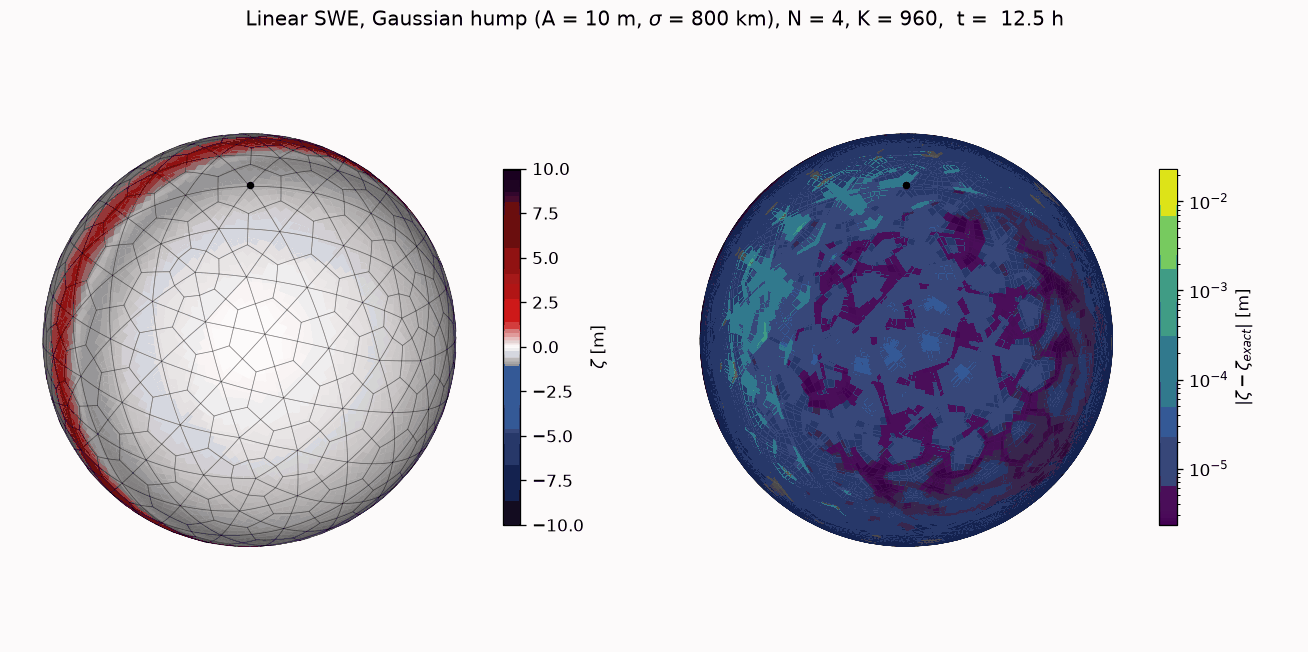
\includegraphics[width=\linewidth]{Figures/GIF_12-5h.png}
        \caption{Snapshot at 12.5h}
        \label{fig:snap12-5}
    \end{subfigure}
    \hfill
    \begin{subfigure}[t]{0.32\linewidth}
        \centering
        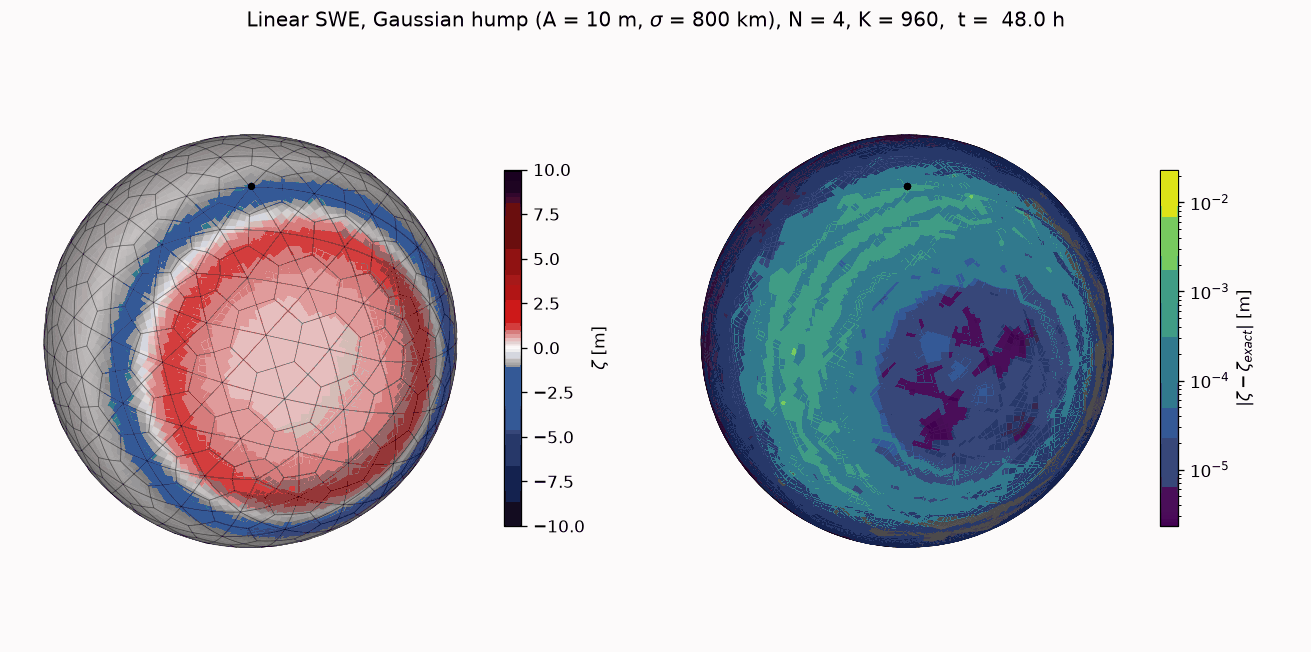
\includegraphics[width=\linewidth]{Figures/GIF_48h.png}
        \caption{Snapshot at 48h}
        \label{fig:snap48}
    \end{subfigure}
    \caption{Snapshots of animation of the wave travelling on the sphere}
    \label{fig:snapshots}
\end{figure}
\section{Future work and outlook}

\newpage
\printbibliography[heading=bibintoc,title={Bibliography}]
\end{document}
